
\begin{exercise}
  State a score theorem for multigraphs. %That is, something like
  \begin{theorem}[Multigraph Score Theorem]
     Let $A = (a_1,\dots,a_n) \in \N_0^n$, $a_1 \geq a_2 \geq \dots  \geq a_n$. There is a multigraph
     with this score if and only if for $A^\prime = (a_1 - 1, a_2 - 1, a_3, \dots, a_n)$has nonegative integers and is multigraphic.

     Furthermore, if $n=1$, then exists a graph with score$(a_1)$ if and only if $a_1=0$.
     If $n=2$, then exists a graph with score$(a_1, a_2)$ if and only if $a_1=a_2$ and $a_1, a_2$ are even.
  \end{theorem}
  
  
  \textbf{Remark.} This is actually
  simpler than for graphs.
\end{exercise}

\begin{exercise}
  Prove your theorem.
\end{exercise}

\begin{proof}
$A^\prime \Rightarrow A$

Obviously, it is true since if $A^\prime$ is a multigraph, a edge is added between the largest two vertices, so $A$ is also a multigraph.

$A \Rightarrow A^\prime$

$A$ has corresponding multigraph and we want to prove that $A^\prime$ also has one.

Let's prove that in $A$, there always exists a multigraph corresponding to $A$ that it has an edge between the vertices of $a_1,a_2$.

If the multigraph corresponding to $A$ has an edge between the vertices of $a_1,a_2$, it's okay.

Else if there is no edge between the vertices $a_1, a_2$. Then there must exist another two vertices connect to them. Suppose the vertice of $a_p$ is connected to $a_1$ and the vertice of $a_q$ is connected to $a_2$.

\textbf{Case 1: $a_p$ and $a_q$ are not the same corresponding vertice.}
\begin{center}
  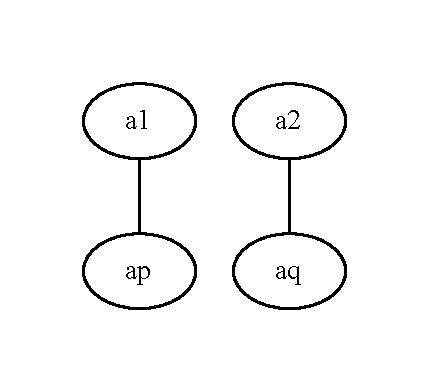
\includegraphics[width=0.3\textwidth]{./figures/7-2-Case1-before.pdf}
\end{center}

We can transform edges $(a_1, a_p)$ and $(a_2, a_q)$ to $(a_1, a_2)$ and $(a_p, a_q)$ ($(a_i,a_j)$ means the edge between the vertices of $a_i$ and $a_j$). It is a new multigraph and it doesn't change the degree of every vertices. So this multigraph is the one we want to find.

\begin{center}
  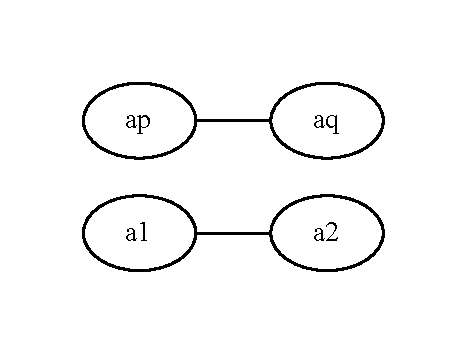
\includegraphics[width=0.3\textwidth]{./figures/7-2-Case1-after.pdf}
\end{center}

\textbf{Case 2: $a_p$ and $a_q$ are the same corresponding vertice.}

\begin{center}
  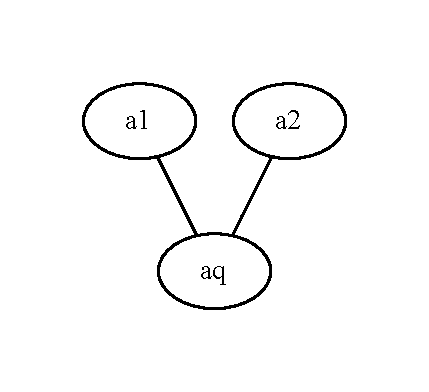
\includegraphics[width=0.3\textwidth]{./figures/7-2-Case2.pdf}
\end{center}

Suppose there are total $u$ edges between the vertices of $a_1, a_p$ and $v$ edges between the vertices of $a_2,a_p$. $u,v \geq 1$

Then $a_1 \geq a_2 \geq a_p \geq u+v$ since the vertice of $a_p$ is connected to at least two vertices.

So the vertices of $a_1, a_2$ have another $v,u$ vertices to connect.

Suppose the vertice of $a_1$ is connected to the vertices of $a_l$ and the vertice of $a_2$ is connected to the vertices of $a_m$.

\textbf{Case 2(a): $a_l$ and $a_m$ are not the same corresponding vertices.}

\begin{center}
  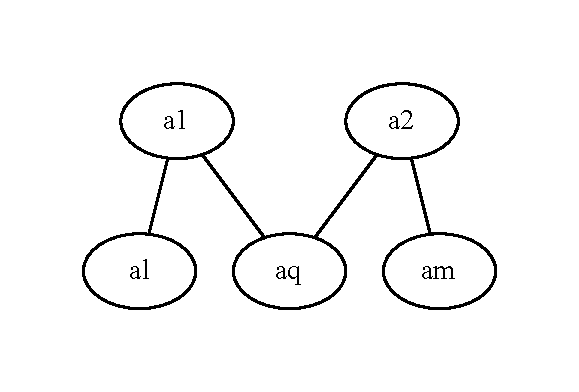
\includegraphics[width=0.3\textwidth]{./figures/7-2-Case2a.pdf}
\end{center}

In fact, it is the same as \textbf{Case 1}. $a_l,a_m$ are the new $a_p, a_q$.

\textbf{Case 2(b): $a_1$ and $a_m$ are the same corresponding vertice.}

\begin{center}
  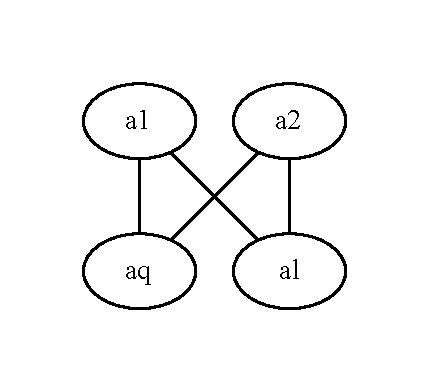
\includegraphics[width=0.3\textwidth]{./figures/7-2-Case2b.pdf}
\end{center}

In fact, it is the same as \textbf{Case 1}. $a_p,a_l$ are the new $a_p, a_q$.

So, in $A$, there always exists a multigraph corresponding to $A$ that it has an edge between the vertices of $a_1,a_2$. And in $A^\prime$, we just reduce one edge between the vertices of $a_1,a_2$. Therefore, $A^\prime$ is also multigraphic.

\end{proof}

